% Sample apostrophy's to remove team's 

\chapter{Grounded Theory}

Constructivist Grounded Theory \cite{Charmaz} provides an iterative approach to data collection, data coding, and analysis resulting in an emergent theory. 

Grounded Theory immerses the researcher within the context of the research subject from the point of view of the research participants. As the research progresses, Grounded Theory allows the researcher to incrementally direct the data collection and theoretical ideas. The theory provides a starting place for inquiry, not a specific goal known at the beginning of the research. As the researcher interacts with the data, the data influences how the research progresses and guides the research direction. When starting a Grounded Theory research study, the core question is, \quotes{what is happening here?} \cite{GlaserTheoreticalSensitivity}. The researcher can apply this question to a domain of study, for example, \quotes{what is happening at the studied organization when it comes to software?}

Charmaz encourages the researcher to \quotes{follow this Grounded Theory strategy: seek data, describe observed events, answer fundamental questions about what is happening, and then develop theoretical categories to understand it.}

%Research questions dictate which research methods are used. Charmaz argues that interviews are the best kind of data collection mechanism for certain kinds of research questions. (Todd: Need more detail)

Grounded Theory allows the addition of new aspects of the research while gathering data, which can even happen late in the analysis. The research question guides the data collection process, and the accumulation of knowledge alters the data collection process. It is common for early research to illuminate new angles. \quotes{Grounded Theory can give you flexible guidelines rather than rigid prescriptions} \cite{Charmaz}. The researcher's guiding interests can be used \quotes{as \quotes{points of departure} to form interview questions, to look at data, to listen to interviewees, and to think analytically about the data} \cite{Charmaz}.

There are three different versions of Grounded Theory: Classic Grounded Theory as championed by Barney Glaser \cite{GlaserDiscovery}, Straussian Grounded Theory as documented by Anselm Strauss and Juliette Corbin \cite{Strauss1988Basics}, and Constructivist Grounded Theory as described by Kathy Charmaz \cite{Charmaz}. 

Barney Glaser and Anselm Strauss invented Grounded Theory while performing the research for the \underline{Awareness of Dying} book \cite{GlaserAwarenessOfDying}. In response to associates asking for more details about the research process utilized in producing the novel results for \underline{Awareness of Dying}, Glaser and Strauss wrote \underline{The Discovery of Grounded Theory} \cite{GlaserDiscovery} in 1967. In 1988, Strauss and Juliet Corbin published \underline{Basics of Qualitative Research} \cite{Strauss1988Basics}. Glaser strongly felt that the book mischaracterized the approach, even asking Strauss to withdraw it from publication. Apparently, both authors had different points of view for what they invented. In a heated response, Glaser published \underline{Basic of Grounded Theory Analysis} in 1992 clearly differentiating his perspective from Strauss. \sout{In time, Glaser's approach became known as \quotes{Classic Grounded Theory} and Strauss's approach as \quotes{Straussian Grounded Theory.}} In time, several researchers evolved the approach using variations (such as recording an interview) that Glaser clearly describes as not part of Classic Grounded Theory. Furthermore, they switched from a positivist point of view to a constructivist perspective. One of these researchers, Kathy Charmaz, a Ph.D. student of Glaser, published \underline{Constructing Grounded Theory} in 2006 \cite{Charmaz}. 

Stol et al \cite{StolGroundedTheory} provide an excellent summary of the differences between the three types of Grounded Theory listed in Table \ref{GroundedTheoryComparison} shown at the end of this section. There are several significant differences which are summarized here:
\begin{itemize}
\item The influence of research questions: emerges from the research (Classic Grounded Theory), may be defined upfront (Straussian Grounded Theory), may be defined upfront and evolves through study (Constructivist Grounded Theory)
\item The role of existing literature: delay in the process (Classic Grounded Theory), use when needed (Straussian Grounded Theory, Constructivist Grounded Theory)
\item Theoretical Coding (Classic Grounded Theory, Constructivist Grounded Theory) versus Axial Coding (Straussian Grounded Theory)
\item Analytic questions: \quotes{what is this data a study of?} (Classic Grounded Theory, Constructivist Grounded Theory), speculating as to causes of the data (Straussian Grounded Theory)
\item Philosophical differences: objectivism (Classic Grounded Theory), pragmatism (Straussian Grounded Theory), and social constructionism (Constructivist Grounded Theory)
\item Evaluation criteria
\end{itemize}

Or

\begin{table}[h]
\centering
\renewcommand{\arraystretch}{1.5}
\caption{Concise comparison of Grounded Theory Approaches}
\label{ConciseGroundedTheoryComparison}
\begin{tabular}{|p{1.3in}|p{1.5in}|p{1.5in}|p{1.5in}|}
\hline
                                    & Classic Grounded Theory                                                                              & Straussian Grounded Theory                                  & Constructivist Grounded Theory                                                                      \\ \hline
The influence of research questions & emerges from the research                                                                            & may be defined upfront                                      & may be defined upfront and evolves through study                                                    \\ \hline
The role of existing literature     & delays use of literature in the process                                                              & use when needed                                             & use when needed                                                                                     \\ \hline
Analytic coding                     & Theoretical Coding                                                                                   & Axial Coding                                                & Theoretical Coding                                                                                  \\ \hline
Analytic questions                  & \quotes{what is this data a study of?}                                                             & hypothesizing as to causes of the data                      & \quotes{what is this data a study of?}                                                            \\ \hline
Philosophical differences           & objectivism                                                                                          & pragmatism                                                  & social constructionism                                                                              \\ \hline
Evaluation criteria                 & fits the data, works in explaining main concern, relevance to participants, modifiable with new data & Seven criteria for process and eight criteria for grounding & credibility (enough data), originality, resonance with participants, usefulness with intepretations \\ \hline
\end{tabular}
\end{table}


Classic Grounded Theory emphasizes action and process. It looks at the question, \quotes{what is going on here?} and decomposes it into \quotes{what are the basic social processes?} and \quotes{what are the basic social psychological processes?} \cite{Charmaz}.

Straussian Grounded Theory relies on Axial Coding as a key differentiator from Glaser's Theoretical Coding. Axial Coding is a systematic process for looking at the relationship between codes for aiding in the emergence of the theory. Axial Coding answers the questions \quotes{‘when, where, why, who, how, and with what consequences} \cite{Strauss1988Basics}. Glaser \cite{GlaserBasics} felt that axial coding favored the six C's  (Causes, Contexts, Contingencies, Consequences, Covariances and Conditions) one of the eighteen theoretical families identified in \underline{Theoretical Sensitivity} without allowing emergence of the other theoretical families \cite{GlaserTheoreticalSensitivity}. Charmaz prefers keeping codes \quotes{simple, direct, analytic, and emergent} instead of applying axial coding which can distract the researcher from understanding what the data means by focusing on the process \cite{Charmaz}. Those in favor of Straussian Grounded Theory see Axial Coding as a more systematic process than Theoretical Coding. 

Constructivist Grounded Theory deviates from Classic Grounded Theory in encouraging the researcher to record and transcribes interviews. Glaser feels that this slows down the research process, overwhelms the researcher with too many codes to analyze, and elicits properline data from the interviewee since they know they are recorded. (Properline data is when interviewees provided information that is socially acceptable for delicate matters. Social norms and corporate narratives reinforce properly aligned data. Glaser is much more interested in understanding what is actually happening. \cite{GlaserAllIsData}.)


The most common technique is interviewing. Interviews are coded and analyzed using constant comparison for the purpose of generating insights and recording memos. The principal activity is creating memos, and it supersedes and interrupts all other activities. The researcher sorts memos into a paper draft with data collection and analysis continuing until theoretical saturation occurs. If a new avenue of research arises,  additional data collection techniques are sometimes useful for generating the needed data. 

\begin{figure}[h]
\centering
\label{GroundedTheoryComparison}
\captionof{table}{Stol's Grounded Theory Comparison}
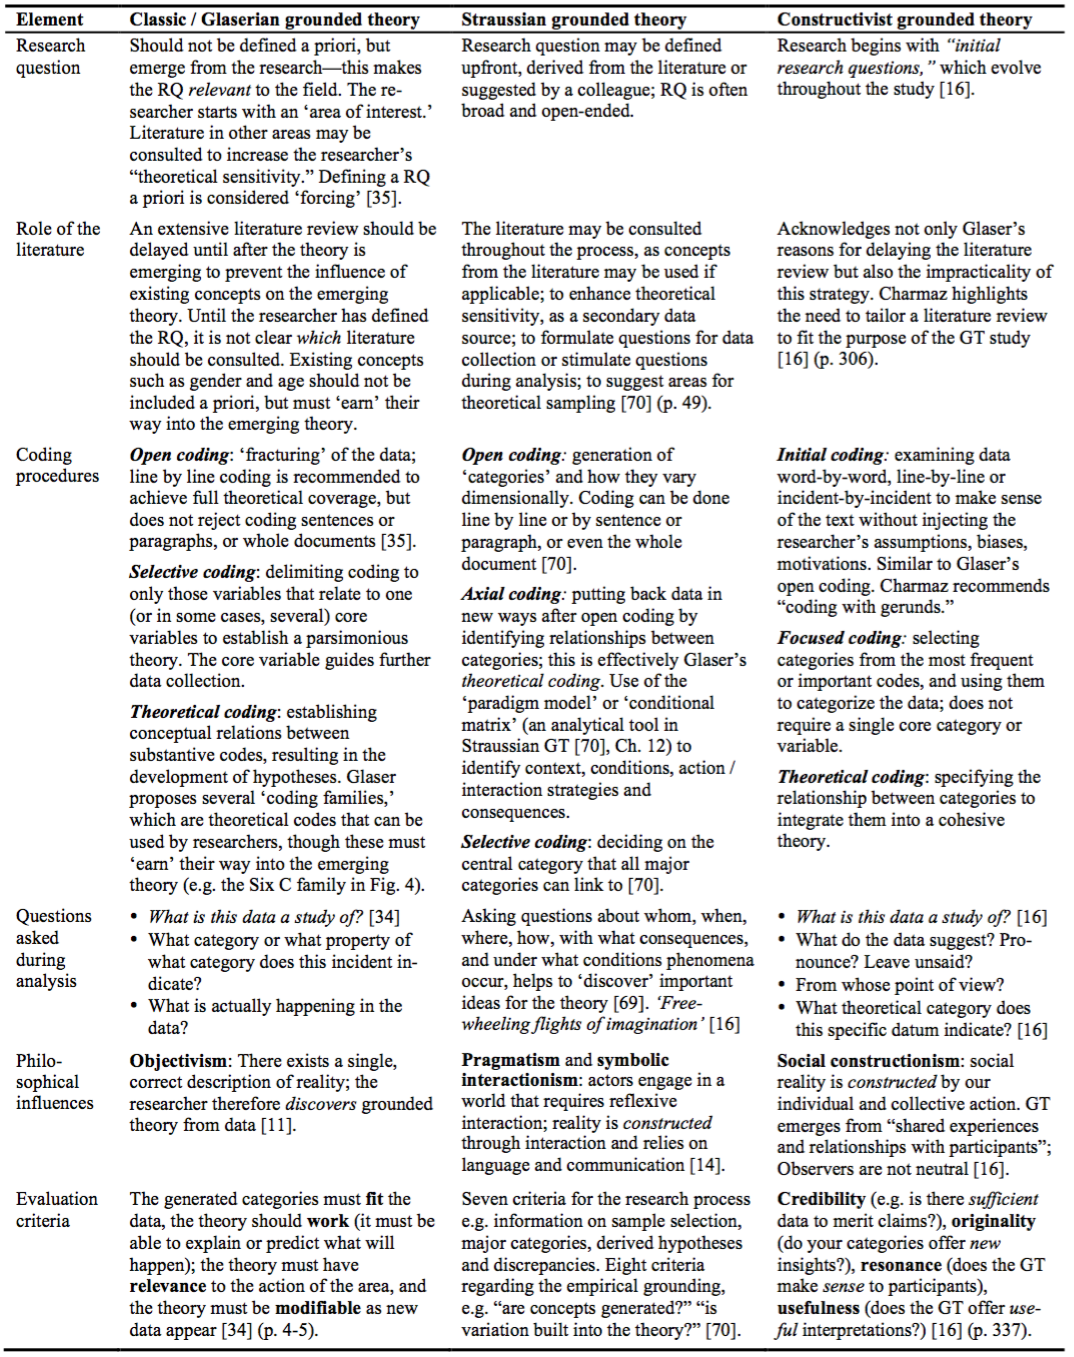
\includegraphics[width=6.4in]{grounded_theory_images/stohl_grounded_theory_comparison.png}
\end{figure}

\section{Interview Technique}
Interviews are the most common technique of gathering data in a Grounded Theory study. Grounded Theory interviews are open-ended explorations of the participant's perspective. Ideally, the interviewer does not force topics but merely follows the path of the interviewee. The interview initially starts with broad, open-ended questions to allow the emergence of unexpected narratives. 

Charmaz suggests \quotes{intensive interviews,} which are \quotes{open-ended yet directed, shaped yet emergent, and paced yet unrestricted} \cite{Charmaz}. Open-ended questions enter into the participant's personal perspective within the context of the research question. The interviewer attempts to abandon assumptions in order to understand and explore the interviewee's perspective. Charmaz \cite{Charmaz} contrasts intensive interviews with informational interviews (collecting facts), and investigative interviews (exposing hidden intentions, practices or policies).

Charmaz describes Glaser and Strauss's approach as \cite{GlaserDiscovery} \quotes{smash-and-grab} by prioritizing the needs of the researcher over the needs of the participants. Instead, she recommends allowing the participant to set the tone and pacing of the interview with the researcher matching and mirroring the participant's tone and pacing. 

The goal is for the researcher to understand the participant's views and actions. The researcher does not need to agree with those views and actions, just interpret them. The researcher can discover what the participants take for granted.

During the interview, the constructivist explores areas of theoretical interest when a participant mentions them. Opening questions slowly guide the conversation towards an area of interest. After understanding what the interviewee's perspective, the researcher can guide the session to provide more detail.

The constructionist endeavors to learn the meanings behind the participant's words or phrases, and not assume that the interviewer and interviewee share a common lexicon, world view, or shared understanding. The constructionist aims to decrease possible preconceptions by understanding the participants' world views. 

The interviewer balances the needs of entering into the interviewee's narrative with getting enough detail to understand the emergent theory. Charmaz argues against placing time limits on interviews. Sometimes it is hard for the interviewer to balance listening to the participant while exploring topics of interest. For example, I thought that one of my interviews was wasteful since the interviewee spent 16 minutes answering one single question. Several times during the interviewee's answer, I was tempted to interrupt. During data analysis, however, this segment turned into a treasure trove. Anxiety might have lead to prematurely moving on and missing interesting data. 

Sometimes asking a follow-up question such as \quotes{could you tell me more or what did you mean by \underline{\hspace{0.8cm}}} will result in the interviewee provided additional, valuable information.

For organizational studies, Charmaz leads in with questions about collective practices and follows up with questions about the interviewee's participation and point of view. For emotionally charged topics, an interview should proceed with safer questions before diving into personally challenging ones. 

When dealing with hard to discuss topics, Charmaz suggests asking the participant \quotes{
could I ask you about \underline{\hspace{0.8cm}}?} instead of being direct with a question such as \quotes{tell me about \underline{\hspace{0.8cm}}?} \cite{Charmaz}. This question reduces the amount of control the interviewer has in the interview by empowering the interviewee.

When ending an interview, Charmaz prefers the question \quotes{is there something?} over a more traditional \quotes{is there anything?} The former assumes that there is something that the person should reveal. The later tends to signal that the interview is ending and tends to close the conversation. I tried the variant, \quotes{tell me one more thing} and it worked well for me.

A Grounded Theory ethnographer can use a recursive interviewing technique by interviewing a participant multiple times. Each subsequent interview resumes the previous conversation and deepens the relationship between the interviewer and the participant. 

Classic grounded theorists argue for note taking during the interview
so that the researcher documents the essentials without getting lost in the details \cite{GlaserTheoreticalSensitivity, GlaserGroundedTheoryPerspective}.  A constructivist finds value in the details. Constructivist grounded theorists argue that recording the interview enables the interviewer to focus on the narrative without worrying about capturing information during the interview. The transcription and coding process delays concerns about what is relevant and allows researchers to make these decisions at their leisure.  

I found that recording the interview, creating a transcript, and coding while listening to the audio helped me identify some of my preconceived ideas. During the coding process, while listening to audio recordings of the interview, I realized that I occasionally misunderstood what the participant said, interpreted what they said in my frame of reference,  or ignored something the participant said that I could have followed up on. Reviewing the interview audio enabled me to become a better interviewer; I now had a feedback loop missing for a classic grounded theorist.

As the research progresses, Grounded Theory allows the researcher to direct the data collection and theoretical ideas incrementally

To summarize, Charmaz describes an \quotes{intensive interview} process. The process involves open-ended questions. The purpose is for the researcher to enter into the participant's personal perspective within the context of the research question. The interviewer needs to abandon assumptions and personal presumptive to understand and explore that of the interviewee. Charmaz contrasts intensive interviews from informational interviews which endeavor to collect accurate \quotes{facts} and investigative interviews that attempt to reveal hidden intentions or expose practices and policies. The participant sets the tone and pacing with the researcher matching. 

\textbf{Interview Guides:} An interview guide is an ordered list of sample questions that the interviewer may use to guide the interview. Interviewers should not see the guides as scripts. The interviewer needs to be present with the interviewee, listening to both verbal and non-verbal communication.

Charmaz advocates that novices rely on interview guides. Creating an interview guide causes the researcher to reflect on sequencing and building of questions, and it reduces the chance of asking leading questions. First, the interview guide serves as a forcing function for the researcher to consider what data they want to collect and the best questions to guide the participant towards those topics. The writing of a guide enables the researcher to consider both how and when to ask difficult questions. Second, relying on an interview guide will decrease the chances of a novice researcher blurting out an inappropriate question, in a moment of panic, or from accidentally asking a leading question. 

Experts tend to internalize the interview guide and follow where the conversion is leading them. The interview guide can help researchers remove their preconceived perspective which might taint questions. Reflecting on the interview guide helps the researcher accomplish their research objectives. 

While grounded theorists agree that researchers should not preconceive the data or the analysis, grounded theorists disagree on what techniques constitute \quotes{forcing} the data. Glasser \cite{GlaserIssues} argues against rules for proper memoing, interview guides, and units for data collection, whereas Charmaz argues that an open-ended interview guide for a semi-structured interview would help prevent novices from accidentally asking loaded questions. 

Charmaz crafts questions to elicit certain kinds of information. For example, \quotes{as you look back on your illness, which events stand out in your mind?} to have participants discuss time sequencing. Glaser might argue that this is forcing the data.  Charmaz believes that it opens up commonplace aspects of life.
\subsection{Interviewing Challenges}
There are potential barriers such as power imbalances, social norms, and prior knowledge, and forcing the data, that may affect the interview process and may affect what participants reveal. 

\textbf{The relationship of the researcher and the participant}, called \quotes{identity} by Charmaz, may affect the interview process. For example, power imbalances of a manager and employee or a professor and students.  Different kinds of strategies can be employed. A researcher could distance oneself from positions of authority: a professor interested in learning techniques may decide to interview students in a different degree program. To alter power imbalance, a domain expert researcher might offer \quotes{personal and professional views to encourage reciprocity} \cite{Charmaz}.

\textbf{Social norms and customs}, called \quotes{etiquette} by Charmaz. Participants might not want to reveal information to a stranger. A company rule of secrecy might make it difficult for a researcher to get the needed information. Framing a question is one way to overcoming this challenge. For instance, asking the question,  \quotes{some people have mentioned having negative pair programming sessions; has that happened to you?} normalizes a negative experience, potentially giving permission to the interviewee to discuss an uncomfortable situation.

\textbf{Prior knowledge} can aid or create difficulties for the researcher. A researcher with domain expertise can know about interesting research questions and how to acquire certain kinds of data. That same domain expertise could blind the researcher to possible explanations that an outsider might see.

\textbf{Preconceived ideas} can be used as starting points for open-ended research. A preconceived idea may inspire a researcher to select an area of passion as long as the data guide them. The key is not to force preconceived ideas onto the data. The researcher can initiate with an interesting idea, yet it is critical for the researcher to be flexible with the research topic, listen to the ideas of the participants, and discover the emergent theory. 

\textbf{Inaccurate interviews} could occur as it is possible for the participant to accidentally or intentionally fabricate their experience. In this case, the researcher may be entering an implicit collusion with their participants \cite{Yanos2008CollusiveObjectification}. Instead of treating such interviews as valueless, Grounded Theorists would examine the interchange trying to understand what is happening which may reveal information about forbidden topics and vulnerabilities of both parties. The after-the-fact analysis may help the researcher from repeating such a performance by understanding how the participant was redirecting the interview. 

\section{Field Notes for Participant Observation or Ethnographic Studies}
The researcher can record observations as field notes, either as a participant involved in the activity or as an ethnographer watching the activity. Recording field notes is complementary to interviewing. 

Field notes might
\begin{itemize}
\item Record individual and collective actions 
\item Contain full, detailed notes with anecdotes and observations 
\item Emphasize significant processes occurring in the setting 
\item Address what participants define as interesting or problematic 
\item Attend to participants' language use 
\item Place actors and actions in scenes and contexts 
\item Become progressively focused on key analytic ideas. \cite{Charmaz}
\end{itemize}

Grounded Theory helps with participant observation and ethnographic studies. \quotes{Grounded theorists select the scenes they observe and direct their gaze within them. Their field-notes show the actions, processes, and events that constitute what is happening in the setting. Grounded Theory methods provide systematic guidelines for probing beneath the surface and digging into the scene. These methods help in maintaining control over the research process because they assist the ethnographer in focusing, structuring, and organizing it} \cite{Charmaz}.

% Asking about specific terms can reveal internal concerns. For example, even with 20 years of software development experience, I had never heard the phrase \quotes{bike-shedding} until a project where several engineers were using it to communicate a concept succinctly. The phrase \quotes{bike-shedding} illustrated that the developers were worried about arguing over trivial matters because the team did not understand the deeper issues. Developers new to a programming language or technology might argue over trivial matters simply because they do not understand which arguments are worth having. Likewise, they might accept solutions because they do not understand the implications.

For an ethnographer, the \quotes{explicit integration of observation and interviewing affords immediate materials for analysis} \cite{Charmaz}. Grounded Theory adds checks and rigor to the ethnographer's data collection and analysis. 

Charmaz provides several questions for ethnographers to understand what they are observing:
\begin{itemize}
\item What are people doing? Which patterns of actions or events do you discern?
\item What strikes you as most noteworthy, most interesting, or most telling?
\item How would you describe the setting( s)?
\item How do hierarchies affect individual and collective actions?
\item What do different participants / groups in the setting seek to accomplish?
\item What do participants' experiences mean to them?
\item How do participants use language?
\item On what criteria do participants and/ or groups judge actions, events, and products or outcomes?
\item To whom are participants accountable?.
\item How do participants explain their actions to each other?
\item How are material resources involved?
\item How do your understandings shift and change as your research proceeds?
\item What theoretical area does this ethnography address? \cite{Charmaz}
\end{itemize}

Collecting and analyzing field notes from participant observation is not easy. At the beginning of her research, Charmaz pictured a research experience where she would observe her research participants during the day and disappear into the coffee room to take detailed notes and write up her experience \cite{Charmaz}. She discovered that this is challenging in practice, as it can be difficult to disappear while observing activities. When the participant activity is intensive, such as the case with pair-programming, recording observations is tricky. I relied on small notes on post-it notes (which were culturally acceptable compared to typing on a laptop) and detailed observations after work.

\section{Documents and other sources of data}
Charmaz suggests that researchers can undervalue documents and encourages researchers to view them as text assets that researchers can mine in the same way as interview notes or field observations. Since the researchers didn't create the document, some might see them  as more \quotes{objective.} 

Charmaz identifies two categories of document, extant documents which exist prior to the researcher's involvement and elicited documents which the researcher creates as the researcher asks participants to answer questions, complete a survey, or write an account of their experiences. With extant documents, the researcher needs to understand the context in which the document is situated. The researcher can use both types of documents to satisfy possible research goals. 

Lindsay Prior \cite{Prior2003UsingDocuments} argues that more than another voice, documents can do things that a participant can not. Beyond \quotes{what do they contain?} the researcher can ask the questions, \quotes{what does the document do?}, \quotes{why was it created?}, \quotes{how was it created?}, \quotes{how are the documents used?}, \quotes{how do people interpret the document?} and \quotes{what is not included in the document?} 
\section{Coding}
The purpose of coding is to fracture the source data into pieces then compare the data against itself during the constant comparison activity. Coding begins the framing from which the researcher builds analysis. In Constructivist Grounded Theory, interviews are recorded, transcribed, and then coded.

Charmaz advises to code everything during the early stages of research and see what emerges. During the initial phase, the researcher should be open to any direction. Once emergent themes arrive, then coding in later parts of the research can be focused around the themes. The focused coding phase allows the researcher to \quotes{sort, synthesize, integrate, and organize large amounts of data} \cite{Charmaz}.

There is no perfect coding scheme. Charmaz prefers one that is simple, short, direct, advice, analytic and spontaneous. Both the researcher's and the participants' vocabulary influences the coding.

There are different styles of coding. Starting with Glasser in 1978 \cite{GlaserTheoreticalSensitivity} some grounded theorists argue for using gerunds (e.g. dealing with uncertainty, exploring solutions to a problem) instead of topic or noun-based coding schemes (e.g. uncertainty, solutions). Relying on gerunds helps encourage the researcher to dig into the data and see the relationship between the participant and their actions. Charmaz strongly argues against labeling events, experiences, or topics as codes as the researcher gains little insight into the participant's meaning, action, or point of view. Because Strauss and Corbin \cite{Strauss1988Basics} places less emphasis on this distinction, many grounded theorists take a more open stance to coding than relying on gerunds.

There are different granularity of coding. Charmaz prefers line-by-line coding and suggests there are times when even word-by-word coding is helpful. The line-by-line coding helps the researcher slow down and examine for nuanced interactions in the data. By 1992, Glasser prefers topic-by-topic or incident-to-incident coding. He advises against decomposing a single indecent. He feels that line-by-line coding produces too many codes, categories, and properties without producing the analysis. While line-by-line coding does generate more codes, I appreciated the intimacy and thoroughness of line-by-line coding.

Charmaz suggests these heuristics to guide the researcher in the coding process:
\begin{itemize}
\item Remain open
\item Stay close to the data
\item Keep your codes simple and precise
\item Construct short codes
\item Preserve actions
\item Compare data with data
\item Move quickly through the data \cite{Charmaz}
\end{itemize}

Charmaz suggests these strategies when examining source materials:
\begin{itemize}
\item Breaking the data up into their component parts or properties
\item Defining the actions on which they rest
\item Looking for tacit assumptions
\item Explicating implicit actions and meanings
\item Crystallizing the significance of the points
\item Comparing data with data
\item Identifying gaps in the data \cite{Charmaz}
\end{itemize}

Whenever insights arise, the researcher immediately stops the coding process and records the insight as a memo.

For the constructivist, the researcher creates the code when the researcher examines the data and finds meaning within it. \quotes{We \textit{construct} our codes because we are actively naming data \ldots We choose the words that constitute our codes. Thus we define what we see as significant in the data and describe what we think is happening} \cite{Charmaz}.

Sometimes a researcher sees everything seems trivial or everything seems significant. This is normal and in time, the data collection and coding process will sort out the core concerns for the participants.

\quotes{The conversation includes more than words alone} \cite{Charmaz}.

When observing routine activity, it can be challenging to see anything meaningful in the data. In this situation, the researcher can compare events to events looking for similarities and differences. 

If for some reason, the codes remain mundane, Charmaz suggests \quotes{coding the codes.} In examining the codes, if there a larger process or activity? Perhaps there are patterns in the codes. 

Tensions may emerge in the coding. Tensions should be embraced rather than avoided or hidden. 

At the researcher codes the data, Charmaz encourages the researcher to answer these questions:
\begin{itemize}
\item What process(es) is at issue here? How can I define it?
\item How does this process develop?
\item How does the research participant(s) act while involved in this process?
\item What does the research participant(s) profess to think and feel while involved in this process? What might his or her observed behavior indicate?
\item When, why, and how does the process change?
\item What are the consequences of the process? \cite{Charmaz}
\end{itemize}

Constructivist Grounded Theory specializes in breaking down phenomena and reflecting on dialog with \quotes{what} and \quotes{how} questions.

\quotes{Grounded theorists aim to code for possibilities suggested \textit{by} the data rather than ensuring complete accuracy \textit{of} the data} \cite{Charmaz}. This stance provides opportunities for checking envisioned ideas with other data. Constant comparison allows the researcher to invalidate conjecture; an errant code will be detected and unsupported by other data samples. Ideas reflected in the data must earn their way into subsequent analysis. Constructivist grounded theorists acknowledge that both the researcher's and the participants' vocabulary influences the coding.

There are two phases of coding: initial coding and focus coding. 

\subsection{Initial Coding}
The initial coding process is where the researcher reads through data such as an interview transcript and marks fragments of data with a summary description or \quotes{interpretive rendering.} The initial coding names every part of the data.  Initial coding is a slowing down process where the researcher becomes intimate with the data. The researcher can examine the data looking for implied things. While the emphasis is on summarizing the data and not analyzing it, the research should record any analysis ideas that could be explored later as memos. The researcher tries to avoid asking what the data means at this stage. Both actions and processes can be coded. The researcher does not want to bring preconceived ideas to coding.

After starting initial coding, constant comparison begins to help shape the direction of the research. 
\subsection{Focused Coding}
Once core categories emerge from constant comparison, the researcher shifts from initial coding to focused coding where the emphasis is flushing out the core categories and their properties. Focused coding continues until theoretical saturation occurs.

\section{Constant Comparison}
Constant comparison allows the researcher to identify \quotes{the conceptual relationship between categories and their properties as they emerged} \cite{GlaserBasics}, leading to an emergent theory.

In constant comparison, the researcher examines and compares codes to each other. It may be the case that two codes should be combined since they are describing the same phenomena. Codes that are related form a category. The researcher compares category to category looking for the relationship between them. The researcher periodically audits each category for cohesion by comparing its codes and moves codes that belong to a different category. Constant comparison compares incident to incident looking for patterns. Similarities strengthen the category while differences refine properties of the category. 

As categories emerge from the data, the researcher is looking for the core category as it defines the chief concern of the participants. Once the core category emerges, the researcher continues to collect and analyze data by examining the properties of the core category and its relationship to other categories until theoretical saturation occurs.

It is possible for the researcher to oscillate between \quotes{seeing data everywhere and nowhere, gathering everything and nothing} \cite{Charmaz}. When this occurs, the researcher returns to the iterative process of collecting, coding, analyzing their data through constant comparison for guidance.

The researcher pauses to record memos for any insights that occur during the analysis.

\section{Memo-writing}
Memo-writing is writing down the researcher's insights and analysis. Memoing can occur at any point in the process, and trumps any other activity.  \quotes{Memo-writing is the pivotal intermediate step between data collection and writing drafts of papers} \cite{Charmaz}. 

Memo-writing pauses the other research activities and allows the researcher to reflect on what is going on in the data and the analysis. Memo-writing encourages the researcher to analyze the data early in the process. The output of memo-writing can enable the researcher to course adjust the research process.

It is normal for memos written early in the research process may be more tentative and less theoretically developed than memos written later in the research process. 

Charmaz encourages the researcher to \quotes{engage an emergent category, let your mind rove freely in, around, under, and from the category; and write whatever comes to you. That is why memo-writing forms an interactive space and place for exploration and discovery. You take the time to discover your ideas about what you have seen, heard, sensed, and coded and then you examine these ideas} \cite{Charmaz}.

Some researchers use a \quotes{Methodological Journal} in which the researcher records dilemma, directions, and decisions. A journal helps the researcher reflect about the data and the process.  The key is for the researcher to find a system that works for them.

For early memos, Charmaz recommends that researchers \quotes{record what they see happening in the data} and to {use early memos to explore and fill out qualitative codes} \cite{Charmaz}. 

For advanced memos, Charmaz suggests to
\begin{itemize}
\item Trace and categorize data subsumed by the topic.
\item Describe how the category emerges and changes. 
\item Identify the beliefs and assumptions that support it. 
\item Specify how the category informs action and experience. 
\item If relevant, tell what it looks and feels like from various vantage points. 
\item Place the category or categories within an argument. 
\item Sharpen comparisons of people, data, codes, categories, subcategories, concepts, and analysis with existing literature. \cite{Charmaz}
\end{itemize}

There is no standard, correct memo. Contents vary from memo to memo. Memos can have a title. Memos tend to be private, unshared documents enabling the researcher to be perfectly free with thoughts, not worrying about grammar, editing, and future readers. The paper writing process will sort all that out. As such, researchers can record doubts, concerns, and first thoughts. Charmaz lists several ways researchers can use a memo:
\begin{itemize}
\item Define each code or category by its analytic properties
\item Spell out and detail processes subsumed by the codes or categories
\item Make comparisons between data and data, data and codes, codes and codes, codes and categories, categories and categories
\item Bring raw data into the memo
\item Provide sufficient empirical evidence to support your definitions of the category and analytic claims about it
\item Offer conjectures to check in the field setting(s)
\item Sort and order codes and categories
\item Identify gaps in the analysis
\item Interrogate a code or category by asking questions of it. \cite{Charmaz}
\end{itemize}

In order to facilitate memo-writing, Charmaz suggests relying on several writing exercises to stimulate the writing process such as freewriting (keep writing whatever comes to the mind, including nonsense) and clustering (diagramming relationships).

Memo-writing can raise focused codes to conceptual categories. As the researcher does the analysis on focused codes, the researcher identifies which codes describe what is occurring in the data. A category can span several codes. 

Both Glaser and Charmaz desire conceptual categories with \quotes{abstract power, general reach, analytic direction, and precise wording} \cite{Charmaz} while grounded in the data. Conceptual categories may be applicable in different domains, professions, and fields and help explain substantive processes. Examples include \quotes{getting off the street} \cite{KarabanowGettingOffTheStreet}, \quotes{managing \textit{spoiled} national identity} \cite{RiveraManagingSpoiledNationalIdentity}, and \quotes{living one day at a time}. Focusing on generic processing raises codes to theoretical categories. 

As the key analytic step, memos become the foundation of the emergent theory.  The researcher may deem some memos as complete whereas others raise unanswered questions. Revisiting previous memos allows the researcher to see what is missing in the memo and directs new research directions. Memo-writing helps the researcher to identify additional data to collect. 

\section{Theoretic Sampling}
Theoretical sampling is collecting additional data to develop full and robust categories, identify the relationships between categories, and flush out the main category's properties. 

For example, data and codes may yield unanswered questions and categories may not be definitive and may suggest new avenues of exploration. Additional data collection, coding, and analysis refine the emergent theory which produces a new vantage point for further exploration and refinement.

Activities include adding new participants, observing in different settings, re-interviewing participants with follow-up questions or ask about different kinds of experiences.

This process continues until the category structure stabilizes and nothing new can be added to the theory, i.e. theoretical saturation. 

Memo-writing spurs theoretical sampling. Theoretical sampling is strategic, specific, and systematic.

Theoretical Sampling is not 
\begin{itemize}
\item Sampling to address initial research questions 
\item Sampling to reflect population distributions
\item Sampling to find negative cases
\item Sampling until no new data emerge. \cite{Charmaz}
\end{itemize}

\strikeout{While Quantitative Researchers aim to have a broad sampling to statistical inferences that describe target populations, qualitative researchers aim to fit their theory to their data. Quantitative researchers aim to test preconceived hypotheses; qualitative researchers aim to generate emergent theories that then become the foundation for new endeavors for quantitative researchers.}

In review, theoretical sampling is collecting additional data to develop full and robust categories, identify the relationships between categories, and flush out the core category's properties.

\section{Memo Sorting}
Memo sorting involves the sorting, comparing, and integrating of the memos to refine the emergent theory. Sorting involves examining different arrangements of the memos to determine which sequence clearly tells the story of the theory. Often memos describing properties of a category are sequenced around the category. If there is a time sequence to a process, memos might be sorted chronologically with the steps of the process. Charmaz suggests printing them out, arranging them on the floor or a dining room table, and rearranging them until a natural progression emerges. Comparing involves juxtaposing two memos and seeing if new insights and thus a new memo emerges. Integrating involves fitting the memos together into a cohesive whole. 

Thus memo sorting is more than simply creating the first draft. The process of memo sorting stimulates additional analytical work, may raise new questions that may stimulate additional data collection, coding, and analysis. 

The memo sorting phase begins the process of helping the researcher articulate the theory.

\section{Theory Construction}
For researchers who do want to generate theory, there are four concerns to attend to theoretical plausibility, direction, centrality, and adequacy. These concerns are the prime concern for the researcher.

Since interviewing allows the researcher to direct and control the data generation, this brings up these theoretical concerns. 

Theoretical plausibility supersedes theoretical accuracy. Charmaz reminds that definitions of accuracy are social constructs. Constructivists express less concern about the accuracy of the participant's point of view than other qualitative researchers.

The amount of data collected in a Grounded Theory study typically offsets any adverse effects of \quotes{misleading accounts} and thus decreases the probability that the research's work would have spurious results. \quotes{Grounded Theory aims to make patterns visible and understandable} \cite{Charmaz}. Thus a grounded theorist should strive to have wide and deep coverage of their categories. 

If a participant does offer exaggerated or inaccurate accounts, and the researcher detects this situation, then this can be a research opportunity into understanding how the candidate is creating fictional representations of their situation. Charmaz recounts seasoned citizens retaining identity patterns from earlier in their life; for example, one person described how she daily attended her garden even though she had not done so for years.

After the initial interviews and the initial coding, a theoretical direction emerges from the data. Certain ideas and codes routinely emerge from the data. The data suggests paths that need exploring.

Once the researcher has explored these paths, theoretical centrality emerges from the coding and analysis. Certain codes become core to the research. The researcher drops less fruitful paths and codes as the researcher focuses the interviews on the central theme or categories. 

During later interviews, the researcher introduces questions to assess the theoretical adequacy of the emergent categories for the purpose of robust theoretical categories. Theoretical adequacy is central to theoretical sampling and saturation. 

Glaser's chief goal is in theory building and routinely emphasizes conceptualization. Theoretical coding requires the researcher to think about the relationship between the codes. Coding families, groups of similar codings, help the researcher consider possible relationships between codes.  In his book, Theoretical Sensitivity \cite{GlaserTheoreticalSensitivity}, Glaser lists 18 theoretical coding families and acknowledges that there may be more:
\begin{enumerate}
\item \textit{The Six C's:} Causes, Contexts, Contingencies, Con- sequences, Covariances and Conditions
\item \textit{Process:} Stages, staging, phases, phasings, progressions, passages, gradations, transitions, steps, ranks, careers, orderings, trajectories, chains, sequencings, temporaling, shaping and cycling.
\item \textit{The Degree Family:} Limit, range, intensity, extent, amount, polarity, extreme, boundary, rank, grades, continuum, probability, possibility, level, cutting points, critical juncture, statistical average (mean, medium, mode), deviation, standard deviation, exemplar, modicum, full, partial, almost, half and so forth.
\item \textit{The Dimension Family:} Dimensions, elements, division, piece of, properties of, facet, slice, sector, portion, segment, part, aspect, section. The dimension family divides the notion of a whole into a parts. 
\item \textit{Type Family:} Type, form, kinds, styles, classes, genre. While dimensions divide up the whole, types indicate a variation in the whole, based on a combination of categories. 
\item \textit{The Strategy Family:} Strategies, tactics, mechanisms, managed, way, manipulation, maneuverings, dealing with, handling, techniques, ploys, means, goals, arrangements, dominating, positioning. 
\item \textit{Interactive Family:} Mutual effects, reciprocity, mutual trajectory, mutual dependency, interdependence, interaction of effects, covariance. 
\item \textit{Identity-Self Family:} Self-image, self-concept, self-worth, self-evaluation, identity, social worth, self-realization, transformations of self, con- versions of identity.
\item \textit{Cutting Point Family:} Boundary, critical juncture, cutting point, turning point, breaking point, benchmark, division, cleavage, scales, in-out, intra-extra, tolerance levels, dichotomy, trichotomy, polychotomy, deviance and point of no return.
\item \textit{Means-goal Family:} End, purpose, goal, anticipated consequence, products.
\item \textit{Cultural Family:} Social norms, social values, social beliefs, and social sentiments.
\item \textit{Consensus Family:} Clusters, agreements, contracts, definitions of the situation, uniformities, opinions, conflict, dissensus, differential perception, cooperation, homogeneity-heterogeneity, conformity, nonconformity, and mutual expectation.
\item \textit{The Mainline Family:} Social control (keeping people in line), Recruitment (getting people in), Socialization (training people for participation), Stratification (sorting people out on criteria which rank them), Status Passage (moving people along and getting them through), Social organization (organizing the people into groups, aggregates and divisions of labor) and Social Order, (keeping the organization of life working normatively), Social institutions (clusters of cultural ideas), Social interaction, (people acting with people), Social worlds (symbolic surround of life), Social mobility (patterned paths of people movement through society) and so forth.
\item \textit{Theoretical Family:} Parsimony, scope, integration, density, conceptual level, relationship to data, relationship to other theory, clarity, fit, relevance, modifiability, utility, condensability, inductive-deductive balance and inter- feeding, degree of, multivariate structure, use of theoretical codes, interpretive, explanatory and predictive power, and so forth.
\item \textit{Ordering or Elaboration Family:} Structural, temporal and generality are the three principal ways to order data.
\item \textit{Unit Family:} Collective, group, nation, organization, aggregate, situation, context, arena, social world, behavioral pattern, territorial units, society, family, etc., and positional units: status, role, role relationship, status-set, role-set, person-set, role partners. 
\item \textit{Reading Family:} Concepts, problems, and hypotheses. 
\item \textit{Models:} Another way to theoretically code is to model the theory pictorially by either a linear model or a property space. \cite{GlaserTheoreticalSensitivity}
\end{enumerate}

\section{Evaluation}
Glaser provides the criteria of fit, work, relevance, and modifiability for determining how well an emergent theory explains the data \cite{GlaserTheoreticalSensitivity}. Stol et al.  \cite{StolGroundedTheory} explain these criteria as:
\begin{itemize}
\item \textbf{Fit}: \quotes{The generated categories must fit the data} 
\item \textbf{Work}: \quotes{It must be able to explain or predict what will happen}  
\item\textbf{Relevance}: \quotes{The theory must have relevance to the action of the area} 
\item \textbf{Modifiability}: \quotes{The theory must be modifiable as new data appear} 
\end{itemize}

Charmaz provides the criteria of credibility, originality, resonance, and usefulness. Stol et al.  \cite{StolGroundedTheory} summarizes these criteria as:
\begin{itemize}
\item \textbf{Credibility}: \quotes{Is there sufficient data to merit claims?} 
\item \textbf{Originality}: \quotes{Do the categories offer new insights?}  
\item\textbf{Resonance}: \quotes{Does the theory make sense to participants?} 
\item \textbf{Usefulness}: \quotes{Does the theory offer useful interpretations?} 
\end{itemize}
\subsection{How much data to collect?}
The researcher continues to gather data until theoretical saturation occurs. At the beginning of a research study, the researcher can not predict when saturation will happen. Thus, there are no useful metrics for how much data to collect. Likewise, it is challenging for a reviewer to determine if a study has collected enough data. Clearly, more data is better than fewer data. Charmaz points out asking how many interviews is enough is asking the wrong question. She would prefer to have enough interviews that strengthen the research with deep and sufficient vigor. 

Studies using mixed methods may require fewer interviews, as the study relies on data from different data sources.

Data should give a full picture. Two key aspects of data for depicting empirical events are suitability and sufficiency.  The researcher needs to plan to gather sufficient data. 

For Glasser \cite{GlaserIssues} and Stern \cite{SternErodingGroundedTheory}, small data samples, and limited data is not an issue since Grounded Theory purpose is to create conceptual categories. Charmaz argues that limited data can lead to weak analysis. 

\subsection{Constructivism}
The Constructivist approach to Grounded Theory \quotes{emphasizes understanding and acknowledges that data, interpretations, and resulting theory depend on the researcher's view} \cite{StolGroundedTheory}. 

The constructivist acknowledges that the \quotes{humanness} of the researcher may affect the research. Constructivists attempt to identify their assumptions and not accidental reproduce the assumptions in the research results. Relying on and listening to the participants helps counteract researcher bias.

The interplay between the researcher and the participant during an interview is particularly interesting from a constructivist perspective. Interviews are situated within a particular context. Changes in location, time, and setting would result in different data.  Charmaz argues that interviews are a construction between the interviewee and the interviewer. \quotes{The result is a construction - or reconstruction - of reality. Through constructing their respective performances, interviewers and interview participants present themselves to each other. However silent, both the interviewer's and participant's performances make and negotiate identity claims} \cite{Charmaz}.

Because Charmaz has a constructivist perspective, she acknowledges that \quotes{neither observer nor observed come to a scene untouched by the world} \cite{Charmaz}. The research method affects the kind of data observed, the researcher's background affects the observations that the researcher can see. The onus is on the researchers to bring scrutiny and reflective practice to understand how their point of view may bias observations. Charmaz points out that \quotes{\textit{people} construct data} through field notes and interviews. While it is tempting to treat an extent report or document as fact, constructivists remind themselves that people collected and formed them.

The contrasting positions of constructivism and positivism made me wonder about my personal stance and how it might affect the research process. While I believe that there are absolute facts to be obtained in fields such as mathematics and the sciences, understanding people is a messy, organic process. For software engineering research, Constructivist Grounded Theory seems aptly suited since software development is a socio-technical endeavor.

\section{Tool Support}
I initially tried various qualitative research tools but found that instead of making me more intimate with the data, they provided a layer of separation. I found digital forms of simple techniques to more effective. I relied on Microsoft word for transcripts, and Google spreadsheets for constant comparison, printing to index cards for key or massive constant comparison.

Since I had a license for NVivo, I experiment with the tool work and eventually decided not to use it. Adding codes was not a streamlined operation. There is no keyboard shortcut to add a code, and there is no auto-complete for existing codes in the system. As the researcher, I had to remember all the codes that I had already added to the system. The cognitive overhead of remembering when to add a new code or re-use an existing code was too much for me. Perhaps the tool would be better for focused coding with a fixed set of codes. Furthermore, the interface to have my advisor review my coding was extremely challenging to use. The existing coding strip implementation needed considerable overhauling.

I also tried Atlas.ti which has keyboard shortcuts and auto-complete suggestions on existing codes creating a better initial coding workflow. I did not like that I could not edit the source material. When I was coding a transcription and noticed an error, there was no way to change the mistake. 

I used Microsoft Word for transcripts and initial coding. I used the three column format. In the third column, I transcribed the interview, breaking sections into new rows. I compulsively recorded the transcripts with timestamps for each segment, although  I maybe once or twice used that information to re-listen to a portion of the interview.  I did initial coding and focused coding in the second column while registering to the audio file. I used the first column for a unique id reference for that row for the purpose of cross-referencing during constant comparison. 

I then exported the word document into a comma separated format with the id and coding columns. I then imported the file into a spreadsheet for constant comparison and analysis. Sometimes constant comparison was easy to do in the spreadsheet. On a few occasions, I printed index cards so that I could physically sort the cards around me. I used mail merge to print specific rows into a Microsoft Word template for Avery shipping labels. After printing the labels, I applied the sticker to color-coordinated index cards. I used one color per data source. After sorting and clustering, I would update the spreadsheet to match the physical arrangement of cards.

At the outset of the research study, I was concerned about efficiently moving through my data. Using a spreadsheet to track constant comparison and flipping back and forth to various word documents, I was worried that it would be inefficient. A tool would allow me just to click on a link. In practice, however, this proved to be not an issue.

\section{Similarities with Agile Software Development and User research}
As an iterative research approach, Grounded Theory shares similarities to agile software development. Both embrace the need for change and start without knowing the final destination. In both, we plan only the next step and adjust our course as we acquire new knowledge and a better understanding of our environment. Just like agile, we need to grow comfortable with ambiguity. 

The approach is similar to Pivotal's Discovery and Framing process for user research. Interaction designers interview prospective users of the system, attempting to create and validate a persona(s). During each interview, the interaction designer writes notes on post-it notes. After a few interviews, the team does a dump and sort, creating buckets by placing post-it notes into groups and performing constant comparison of each bucket. Key insights are noted. User research is a pragmatic version of Grounded Theory that allows the researcher to explicitly test preconceived ideas and assumptions using explicit questions to force certain topics into the conversation.  Grounded Theory prefers much more open-ended questions that do not force the data. User research tends to rely on a smaller number of interviews to achieve key insights. 
User research is a pragmatic process attempting to identify easy-to-find insights, not generate an exhaustive theory, and thus fewer interviews seem necessary.



\section{Summary}
Starting a Grounded Theory research study, the researcher asks the core question is \quotes{what is happening here?}  \cite{GlaserTheoreticalSensitivity}

Grounded Theory allows the researcher to include new aspects of the research while gathering data and can even happen late in the analysis. The data collection process is guided by the research and altered as knowledge is accumulated. It is common for early research to illuminate new angles. \quotes{Grounded Theory can give you flexible guidelines rather than rigid prescriptions} \cite{Charmaz}. The theory provides a starting place for inquiry, not a specific goal known at the beginning of the research. The researcher's guiding interests can be used as points of  \quotes{departure to form interview questions, to look at data, to listen to interviewees, and to think analytically about the data} \cite{Charmaz}.

After interviewing, data analysis begins with line-by-line coding as recommended by Charmaz \cite{Charmaz}. Coding line-by-line helps the researcher identify nuanced interactions in the data and avoid jumping to conclusions. The data then advanced from these initial codes to focused codes, focused codes to core categories, and core categories to an emergent theory. 


